
\documentclass[a4j,10pt]{jsarticle}
\usepackage{layout,url,resume}
\usepackage[dvipdfmx]{graphicx}
\pagestyle{empty}

\begin{document}
%\layout

\title{[TERM]RGBカメラによる自律飛行経路探索手法の提案}

% 和文著者名
\author{
    著者その1 \thanks{井手田 悠希}
}

% 和文概要
\begin{abstract}
現時点で安価で広く流通している上に小型のものも多く存在するRGBカメラによる自律飛行経路探索手法を提案する.また,本研究では障害物が多く存在する屋内でのランダムウォークを第一段階の目標とし.また,これらに加えて本研究では人物追従や他のドローンの追従,追従しているドローンによる被追従ドローンの制御を目標最終的な到達目標としている.
\end{abstract}

\maketitle
\thispagestyle{empty}

\section{はじめに}
ドローンを映像で制御していくことの今後の展望として,ドローンの第三者視点映像による高精度制御がある.これは物資輸送を行う際に,複数機体のメンテナンスや冗長性を考慮して保有機種を少なくする為に,大型の物資は複数の中型機で輸送し,それ以外は1機で輸送したい.
これらを実現する上で複数ドローンが密集した状態での高精度制御が要求される.その前段階の技術として,ドローンを外部の映像によって制御することを実現したい.

\section{背景}
2010年頃からParrot社による家庭用ドローンの発売などもあり,これ以降ドローンの認知と研究開発は加速している.
付随して,自律飛行に関しても研究が盛んに行われているが,現在行われている自律飛行ではLIDARなど他のセンサーと比較して高価なものを使用している例が多い.また広く流通しているものは大きいものばかりである.これらの問題はドローンでの活用がさらに進めばセンサー自体の開発も進み解決するだろう.しかし,LIDAR等のセンサー以外を主とした飛行経路探索手法を模索することは今後の自律飛行の精度向上に貢献すると考え,本研究を実施するに至った.

\subsection{hoge}

\begin{enumerate}
\item 番号付き箇条書き 
\item 番号付き箇条書き
\end{enumerate}

\begin{itemize}
\item 箇条書き
\item 箇条書き
\end{itemize}

%---------------------------------------------

\section{研究目的}

\subsection{hoge}
hogehoge
画像を貼って見た

\begin{figure}[htbp]
    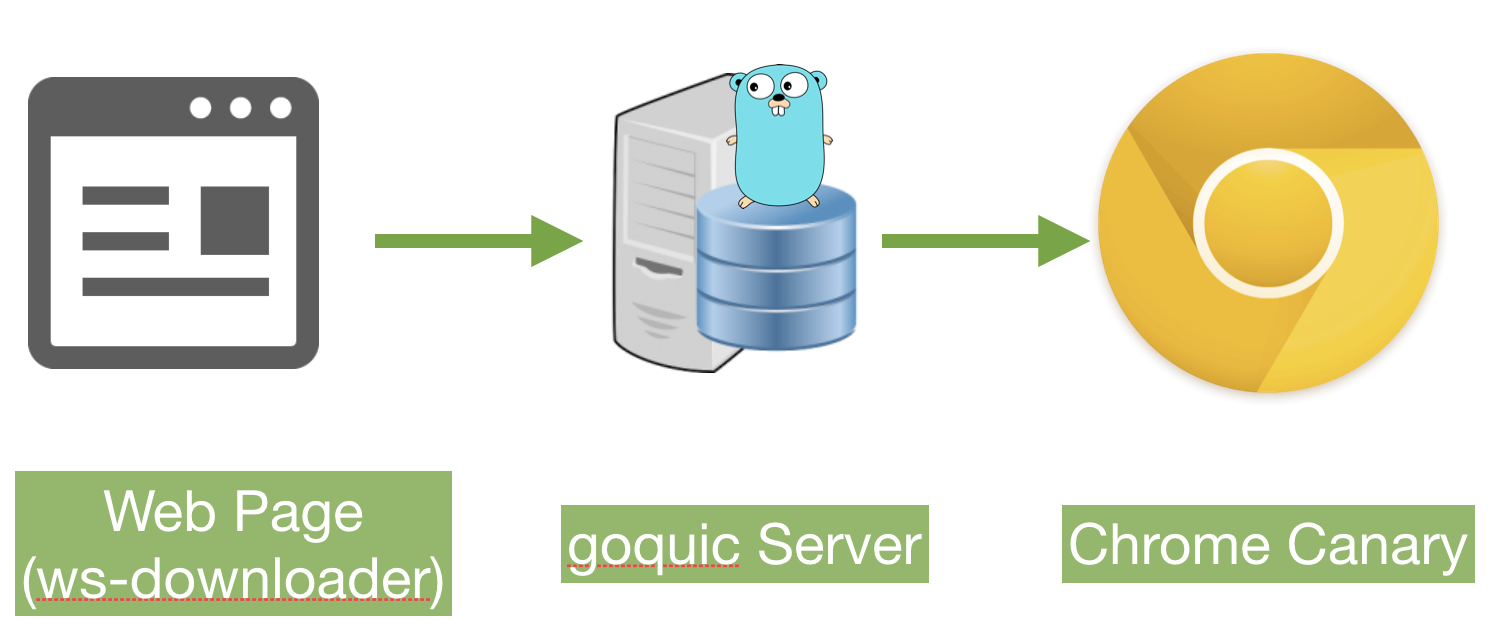
\includegraphics[width=5cm]{figure1.png}
    \caption{}
\end{figure}
 
\subsection{fuga}
fugafuga

\section{関連研究}

\section{提案手法}

\section{評価}

\section{考察}

\begin{thebibliography}{99}
%\bibitem{a}
\bibitem{example}
引用その1\\
\texttt{ http://www.example.com}
\end{thebibliography}

\end{document}
% end of file
